\newpage
\chapter*{Simulations}
\addcontentsline{toc}{chapter}{Simulations} 




% Reconsider later if some if this is better placed in methods section
% or under different title
\section*{Frictional properties of the intact graphene sheet}
The friction measurment simulation is governed by the following parameters, which is divided into three sub categories for the purpose of this thesis as shown in table \ref{tab:param}.



\begin{table}[H]
  \begin{center}
  \caption{Parameters of the numerical procedure for measuring friction.}
  \label{tab:param}
  \begin{tabular}{ | c | m{8cm}| m{5cm}|} 
    \hline
    Category & Parameter name: description & Category purpose \\ 
    \hline
    Physical & 
    \begin{itemize}
      \item[-] T: Temperature for the Langevin thermostat.
      \item[-] $v_{drag}$: Drag speed for the sheet translation.
    \end{itemize} &
    Parameters that we expect to have an inevitably effect on the system friction properties, for which the choice will be a baseline for our studies.
    \\ \hline
    Measurement & 
    \begin{itemize}
      \item[-] $dt$: Integration timestep.
      \item[-] $t_R$: Relaxtion time before strething.
      \item[-] Pauses between stretch and adding normal force and between dragging the sheet.  
      \item[-] Stretch Speed: How fast to stretch the sheet.
      \item[-] $K$: Spring constant for the spring responsible of translating the sheet. An infinte spring constant is achieved by moving the end blocks as a rigid body (Lammps: fix move).
      \item[-] Drag Length: How far to translate the sheet.
      \item[-] Sheet size: Spatial size of the 2D sheet.  
    \end{itemize} &
    Paramters that effects the simulation dynamics and the 'experimental procedure' that we a mimicking. We aim to choose to these paramters such that the friction properties is stable for small perturbations.  \\ \hline
    ML input & 
    \begin{itemize}
      \item[-] Sheet configuration: A binary matrix containing information of which atoms is removed (0) and which is still present (1) in the graphene structure.
      \item[-] Scan angle: The direction for which we translate the sheet.
      \item[-] Stretch amount: The relative sheet stretch in percentage.
      \item[-] $F_N$: Applied normal force to the end blocks.
    \end{itemize} &
    The ramaining paramters that serve as the governing variables in the optimization process for certain friction properties and is thus the input variables for the ML part. 
    \\ \hline
  \end{tabular}
  \end{center}
\end{table}


We should try to set the physcis and measurement parameters in such a way that we reduce computation speed where it is doesn't infer with the frictional properties study.

We need to define some ranges for the ML input paramters. $F_N$, stretch ranges where it is not prone to ruptures. The configuration it self does not have clear rules but is also being regulated by the no rupture requirement. 

Retardation effects due to the finiteness of the speed of sound are usually irrelevant in slow-speed experiments (v < 1 mm/s) \cite{Manini_2016}

In macroscopic tribology experiments, sliding speeds often range in the 0.1 − 10 m/s region \cite{Manini_2016}

By contrast, in nanoscale AFM experiments the tip usually advances at much lower speeds ≃ 1 μm/s: over a typical run it is possible to simulate a tiny ∼ 1 pm displacement, far too small to explore even a single atomic-scale event, let alone averaging over a steady state.\cite{Manini_2016}


However, MD simulations can provide so much physical insight that they make sense even if carried out at much higher speeds than in real-life AFM or surface force apparatus (SFA) experiments: in practice, currently the sliding speeds of most atomistic tribology simulations are in the ∼ 1 m/s region.\cite{Manini_2016}


Besides the limitations of system size and simulation times that are obvious and will be discussed later, there is another limitation concerning temperature, that is rarely mentioned. All classical frictional simulations, atomistic or otherwise, are only valid at sufficiently high temperature. They become in principle invalid at low temperatures where the mechanical degrees of freedom of solids progressively undergo ”quantum freezing”, and both mechanics and thermodynamics deviate from classical. \cite{Manini_2016}.

\newpage
\subsection{Baseline}

\subsubsection{Single measurement}
\paragraph*{Force oscillations}

We first assess the raw data for the friction force $F_{\parallel}$ parallel to the drag direction as seen in figure \ref{fig:drag_Ff}. The sample rate is 10 ps$^{-1}$ for which we sample the the mean of all previous timesteps. We observe that the data carriers oscillations on different time scales. By applying a savgol filter to data with a polyorder of 5 and window length corresponding to a drag length of 3.0 Å (or time interval 15.0 ps) we can qualitatively point out at least two different frequencies of osccilation. On figure \ref{fig:drag_Ff_10} we see roughly three waves on the savgol filter corresponding to one frequency, while on \ref{fig:drag_Ff_100} the same savgol filter reveals an even slower frequency on top of the first creating a visual patterns of a wavepacket.

\begin{figure}[H]
  \centering
  \begin{subfigure}[b]{0.49\textwidth}
      \centering
      \includegraphics[width=\textwidth]{figures/baseline/drag_Ff_10Å.pdf}
      \caption{Drag length of 10 Å.}
      \label{fig:drag_Ff_10}
  \end{subfigure}
  \hfill
  \begin{subfigure}[b]{0.49\textwidth}
      \centering
      \includegraphics[width=\textwidth]{figures/baseline/drag_Ff_100Å.pdf}
      \caption{Drag length of 100 Å.}
      \label{fig:drag_Ff_100}
  \end{subfigure}
  \hfill
     \caption{Friction force $F_\parallel$ between (full) sheet and substrate with respect to the drag direction vs. drag length. The drag length is measured by the constant movement of the virtual atom and not the COM of the sheet. The red line represents a savgol filter with window polyorder 5 and windoew length 150 (corresponding to a drag length of 3 Å or a time window of 15 ps)}
     \label{fig:drag_Ff}
\end{figure}

By performing a Forward Fourier Transform of the data (using FFT) we can quantitavely idendity some of the leading frequencies as seen in figure \ref{fig:ft_a}. By plotting the two most dominant frequencies $f_1 = 0.0074$ ps $^{-1}$ and $f_2 = 0.0079$ ps $^{-1}$ as $\sin{(2\pi f_1)} + \sin{(2\pi f_2)}$ we find a convincing fit to the observed wavepacket shape as seen in figure \ref{fig:ft_b}. By using the trigonometric identity

\begin{align*}
\sin (\alpha+\beta) &= \sin (\alpha) \cos (\beta) + \cos (\alpha) \sin (\beta), \\
\sin (\alpha-\beta) &= \sin (\alpha) \cos (\beta) - \cos (\alpha) \sin (\beta),
\end{align*}
and decomposing $f_1 = a - b$, $f_2 = a + b$ we can rewrite the sine sum as the sinusoidal product
\begin{align*}
  \sin(2\pi f_1) \sin(2\pi f_2) &= \sin(2\pi (a - b)) \sin(2\pi (a + b)) \\
  &= \sin(a)\cos(b) + \cancel{\cos(2\pi a)\sin(2\pi b)} + \sin(2\pi a)\cos(2\pi b) - \cancel{\cos(2\pi a)\sin(2\pi b)} \\
  &= 2 \sin(2\pi a) \cos(2\pi b),
\end{align*} 

with 
\begin{align*}
  a = \frac{f_1 + f_2}{2} &= 0.0763 \pm 0.0005 \text{ps}^{-1},& 
  b = \frac{f_2 - f_1}{2} &= 0.0028 \pm 0.0005 \text{ps}^{-1},& \\
  &= 0.381 \pm 0.003 \text{Å}^{-1},& 
  &= 0.014 \pm 0.003 \text{Å}^{-1},& 
\end{align*}

where the latter frequency is denoted with respect to drag length. This makes us recognize the fast osccilation frequency as $a$ and the slower frequency as $b$. We also take note of the longest period in the data $T_b = 1/b \sim 357$ ps $\sim 71$ Å$^{-1}$ which will be relevant for the evaluation of measurement incertainty.



\begin{figure}[H]
  \centering
  \begin{subfigure}[b]{0.49\textwidth}
    \centering
    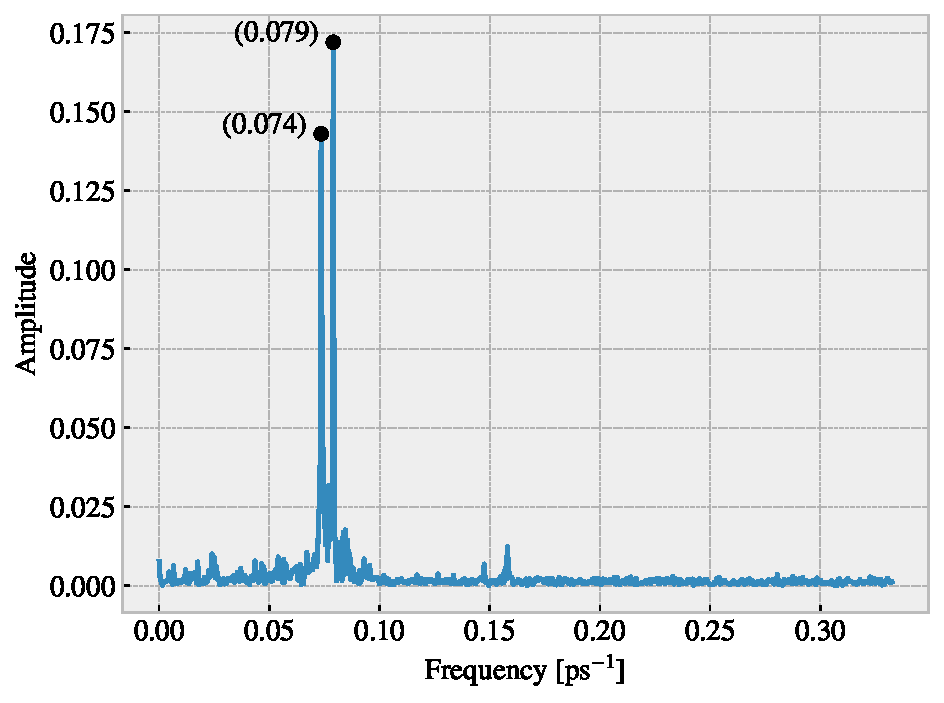
\includegraphics[width=\textwidth]{figures/baseline/ft_zoom.pdf}
    \caption{Reduced frequency range.}
    \label{fig:ft_a}
  \end{subfigure}
  \hfill
  \begin{subfigure}[b]{0.49\textwidth}
      \centering
      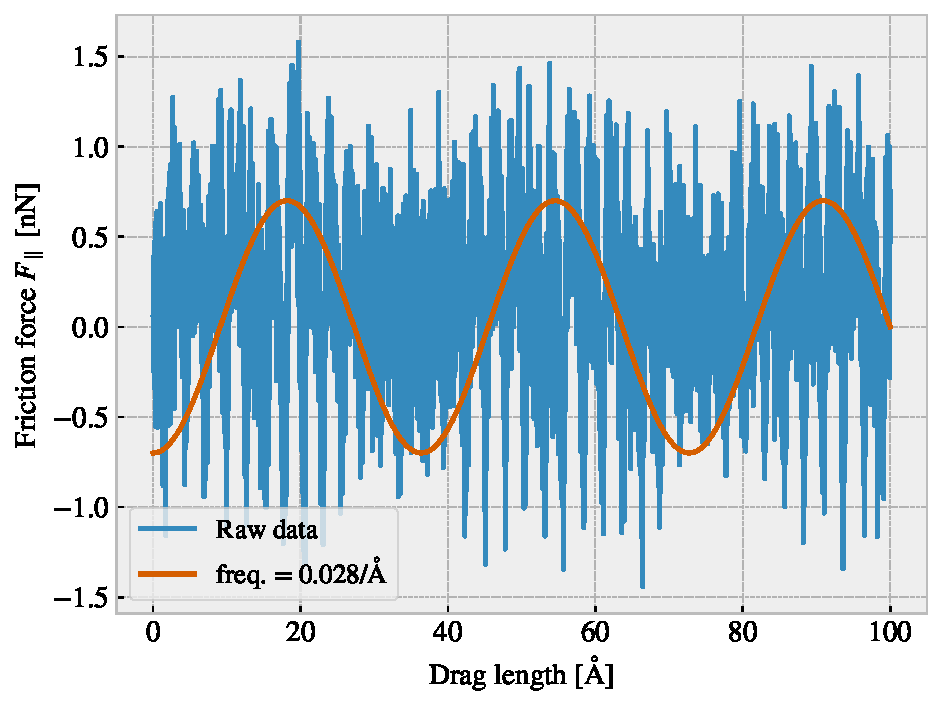
\includegraphics[width=\textwidth]{figures/baseline/ft_sine.pdf}
      \caption{Selected frequencies applied to data from figure \ref{fig:drag_Ff_100}}
      \label{fig:ft_b}
  \end{subfigure}
  \caption{Fourier transform on data shown in figure \ref{fig:drag_Ff}.}
  \label{fig:ft}
\end{figure}


\paragraph*{Decompositions}

In the previous analysis we have looked only as the friction force for the full
sheet, including the pullblocks which is locked off during the drag, and with
respect to the drag direction. \par
Since we are only applying cuts to the inner sheet (excluding the pull blocks),
it might seem more natural to only consider the friction on that part. If the
desired frictional properties can be observed from the inner sheet we can always
scale the relative size between inner sheet and pull block. However, when
looking at the time series of friction force decomposed onto inner sheet and
pull block (figure \ref{fig:decomp_group}) we observe the friction force arrising
from those parts is seemingly antisymmetric. That is, the fricitonal pull on the
substrate is oscillating between the inner sheet and the pullblock. Remembering
that the normal forc eis only applied to the pull block we might take this as an
integrated feature of the system. An interesting nonlinear friction coefficient
might depend on this internal distribution of forces. Hence, we hedge our bets and
use the full sheet friction force as hollistic approach to the measurement problem.

\par
Similar we might question the decision of
only considering the frictional force projected on the direction of the drag as
we are neglecting the ``side shift'' induced during the drag phase. In figure \ref{fig:decomp_direc} we see the decomposition into force components parallel $F_{\parallel}$ and perpendicular $F_{\perp}$ to the drag direction respectively. We see that the most dominant trends is projected into the parallel component. If we want to include the perpendicular component as well we would have to evaluate the friction as the length of the vector for which we loose the sign of direction. Hence we would only get positive contributions, meaning a resisting force, which is not faithfully capturing the sheet oscillaitons that make the friction forces act both against in with the direction of drag. By this argument we decide to use only the parallel component going forward. 

\begin{figure}[H]
  \centering
  \begin{subfigure}[b]{0.49\textwidth}
    \centering
    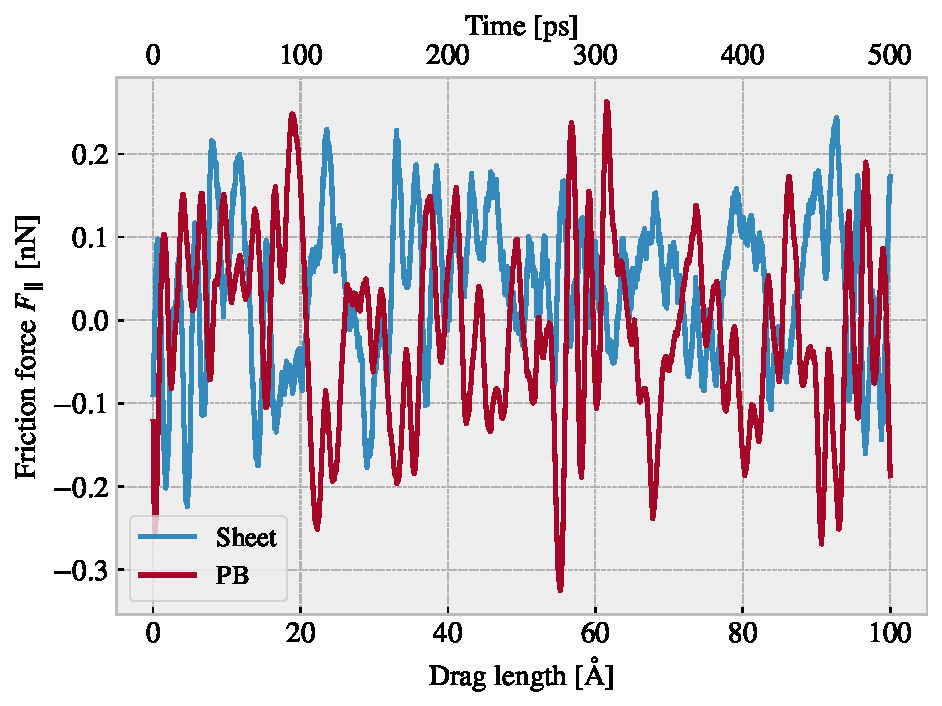
\includegraphics[width=\textwidth]{figures/baseline/decomp_group.pdf}
    \caption{Decomposition into group inner sheet (sheet) and pull blocks (PB).}
    \label{fig:decomp_group}
  \end{subfigure}
  \hfill
  \begin{subfigure}[b]{0.49\textwidth}
      \centering
      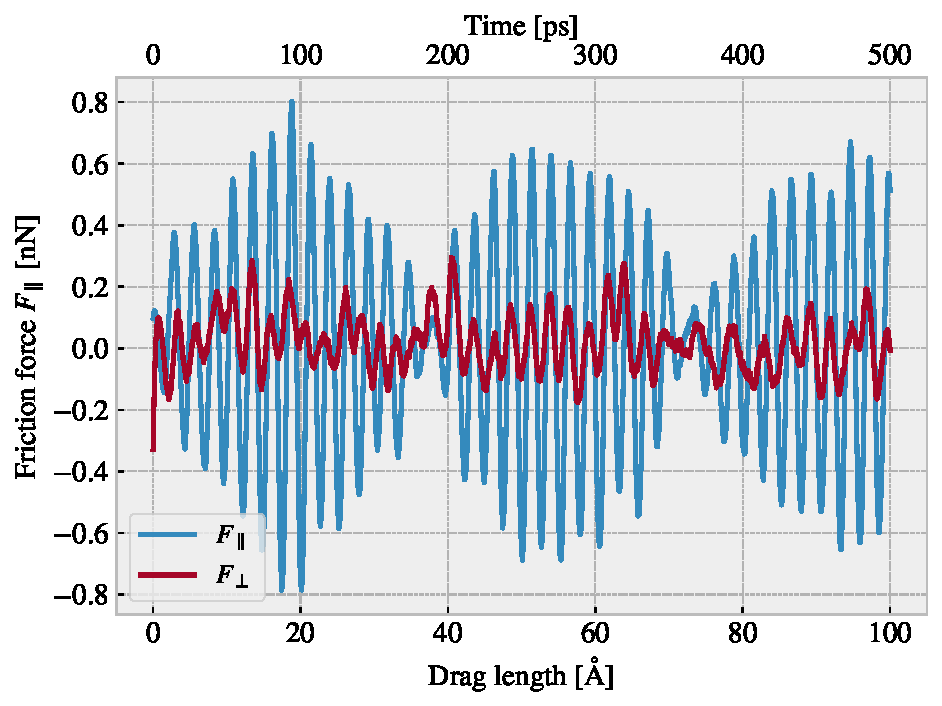
\includegraphics[width=\textwidth]{figures/baseline/decomp_direc.pdf}
      \caption{Decomposition into parallel ($\parallel$) and perpendicular $(\perp)$ to drag direction.}
      \label{fig:decomp_direc}
  \end{subfigure}
  \caption{Decomposition into parallel ($\parallel$) and perpendicular $(\perp)$ to drag direction showing the savgol filter applied}
  \label{fig:decomp}
\end{figure}


\paragraph*{Center of mass path}

From the previous observations we already have evidence of a stick slip behaviour, judging from the friction oscillations in figure \ref{fig:drag_Ff}, and motion partial motion perpendicular to the drag direction, judging from the perpendicular force component in figure \ref{fig:decomp_direc}. By looking at the $x,y$-position for the center of mass (COM) we can see the stick slip motion manifested as a variation in COM speed combinned with a side to side motion as shown in figure $\ref{fig:COM_path_K0}$. To increase this effect we also show the same plot with a spring ... move with spring constant 30 N/m in figure \ref{fig:COM_path_K30}. While the max speed is on the same scale the side to side motion is increased (notice that the axis scale is different between figure \ref{fig:COM_path_K0} and \ref{fig:COM_path_K0}).


\begin{figure}[H]
  \centering
  \begin{subfigure}[b]{0.85\textwidth}
    \centering
    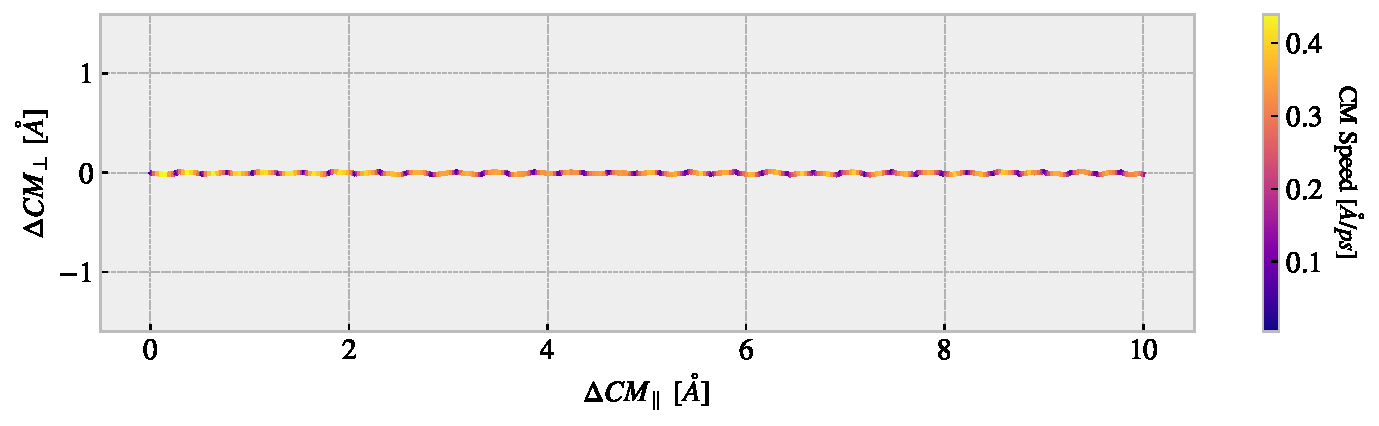
\includegraphics[width=\textwidth]{figures/baseline/COM_path_K0.pdf}
    \caption{Fix move}
    \label{fig:COM_path_K0}
  \end{subfigure}
  \hfill
  \begin{subfigure}[b]{0.85\textwidth}
      \centering
      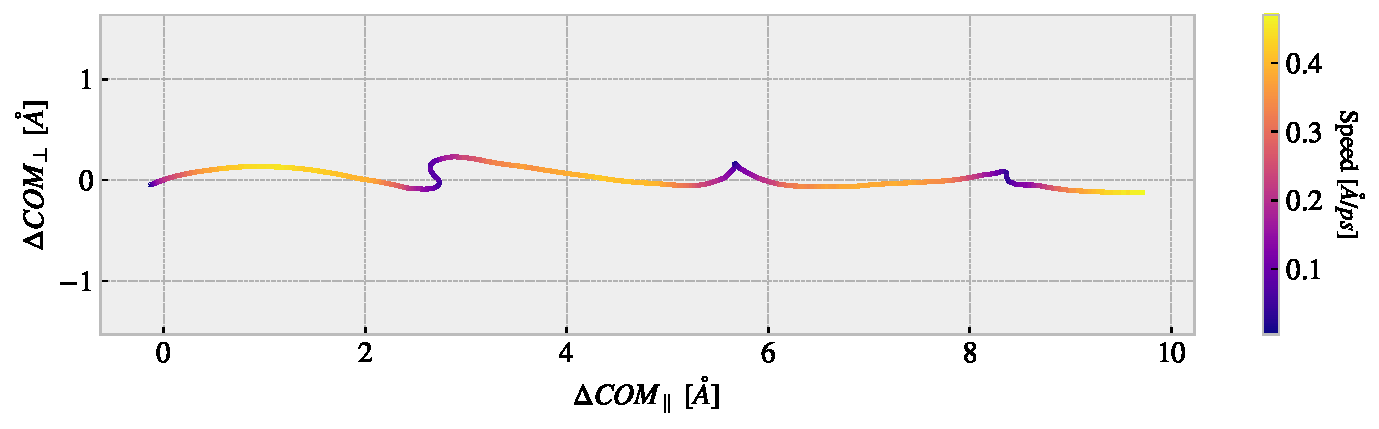
\includegraphics[width=\textwidth]{figures/baseline/COM_path_K30.pdf}
      \caption{K = 30}
      \label{fig:COM_path_K30}
  \end{subfigure}
  \caption{Center of mass relative position from start of drag phase in terms of axis parallel to drag direction $\Delta COM_{\parallel}$ and axis perpendicular to drag direction $\Delta COM_{\perp}$. The colorbar denotes the absolute speed of the COM.}
  \label{fig:COM_path}
\end{figure}




\subsubsection{Defining metrics for dynamic and static friction}
We are interested taking the comprehensive friction force time series dataset
and reducing it into single metrics describing the dynamic and static friciton
respectively. The natural choice is to use the mean and max values. 

\paragraph*{Dynamic friction} For the dynamic friction measurement we take the mean of the latter half of the data to ensure that the system has
stabilished itself before taking the mean. For a full drag simulation of 400 Å
we would thus base our mean value on the latter 200 Å drag. In figure
\ref{fig:runmean} we have shown the friction force of the first 10 Å of drag
together with a running mean with window length 50\% of the corresponding data
length. The final mean value estimate is indicated with red point at the end and
we clearly observe that the length of sampling is insufficient since we ger a
negative friction force.  Nonetheless, one approach to quanity the uncertainy of
the final mean estimate is to consider the running mean. The more the running
mean fluctuates the more uncertainty is associated with the final estimate. 

% That is, if the running mean is constant it doesn't really matter whether we
% stop early or drag a bit longer. However, any fluctuations of this line means
% that out mean measurement is still sensitive to the drag length and any
% changes in the simulation inducing a phase shift of this oscillations will
% effect the final mean value in unaccountable manner. 

We should not care for flucations in the initial part of the running mean curve
as this is still including data from the beginning, where it might transistion
from static to dynamic friction. Only the running mean ``close'' to the ending
should be considered for our uncertainty. From the Fourier analyse we concluded
that longest period of any dominant oscialltions is $\sim 71$ Å$^{-1}$
corresponding to $\sim 35 \%$ of the running mean window of 200 Å drag. Hence we use use standard deviation of the final 35\% of the running mean curve to approximate the uncertainty of the final mean value. By dividing with the final running mean we effectively calculate the relative error as shown in figure \ref{fig:runstd}. Naturally, we get a relative error of $\sim 257\%$ which corresponds with the mean value taking an unexpected negative value.


\begin{figure}[H]
  \centering
  \begin{subfigure}[b]{0.49\textwidth}
    \centering
    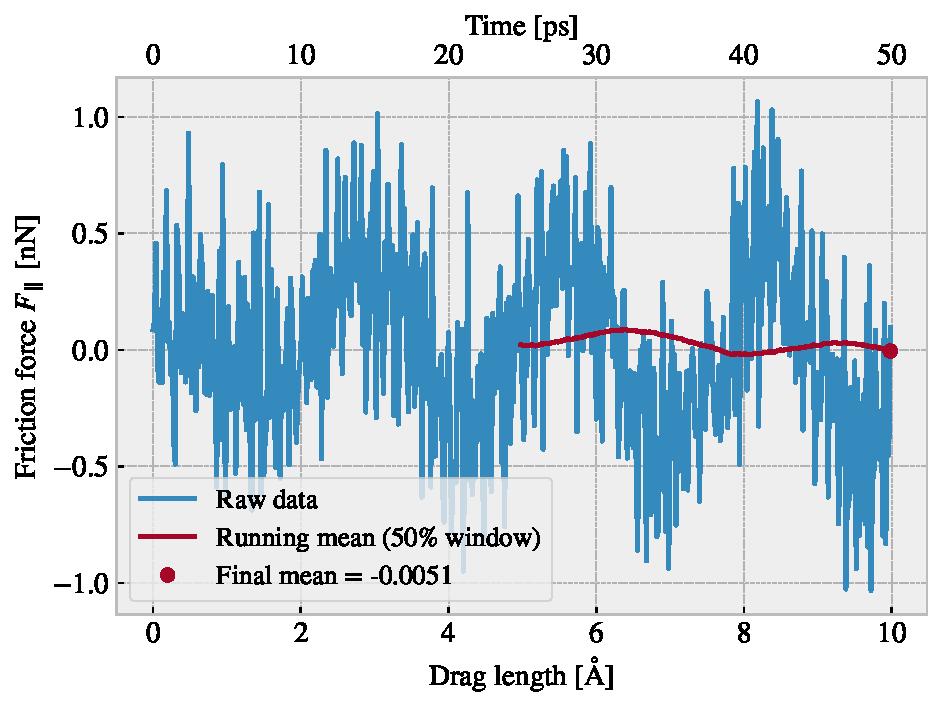
\includegraphics[width=\textwidth]{figures/baseline/Ff_runmean.pdf}
    \caption{Running mean}
    \label{fig:runmean}
  \end{subfigure}
  \hfill
  \begin{subfigure}[b]{0.49\textwidth}
      \centering
      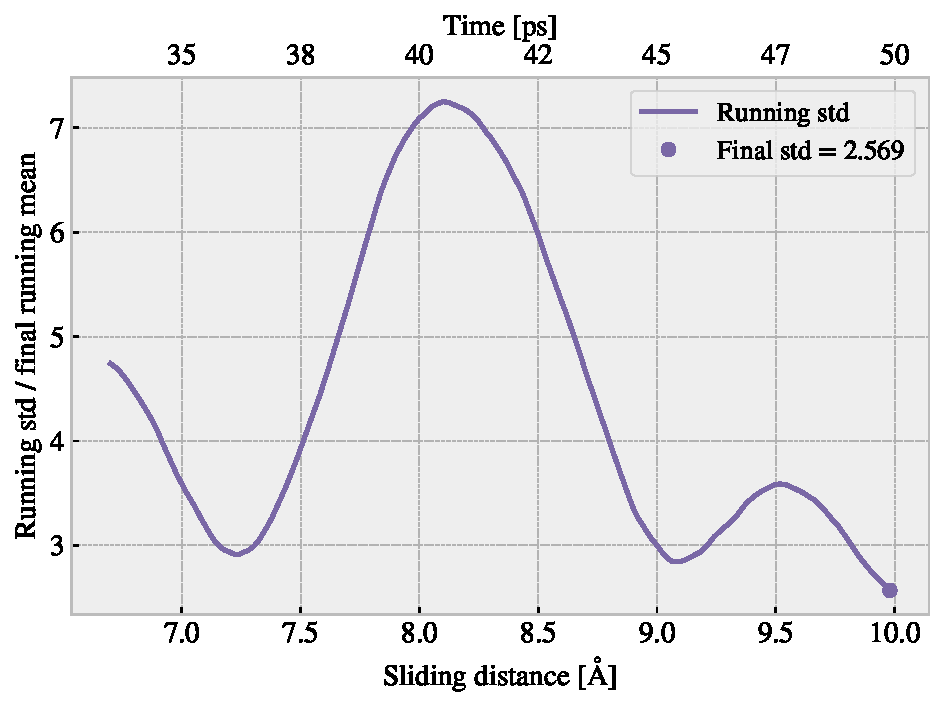
\includegraphics[width=\textwidth]{figures/baseline/Ff_runstd.pdf}
      \caption{Running std}
      \label{fig:runstd}
  \end{subfigure}
  \caption{Running std}
  \label{fig:running}
\end{figure}

When we include the full 400 Å drag, such that std window actually matches with the longest period of oscillations expected from the data, we get a final relative. error of $\sim 12 \%$ as shown in fig \ref{fig:runstd_long}. This is just at the limit for an acceptable error, but as we shall see later (refer to figure or something) this high error is mainly connected to the cases of low friction. When changing the simulation parameters, such that the mean friction evaluate to considerable higher values, the relative error drops to around (put in numbers). One explanation is that the osccilations in the running mean does not increase linearly with the magnitude of the friction, and hence the relative error might spike especially for the low friction cases. 


\begin{figure}[H]
  \centering
  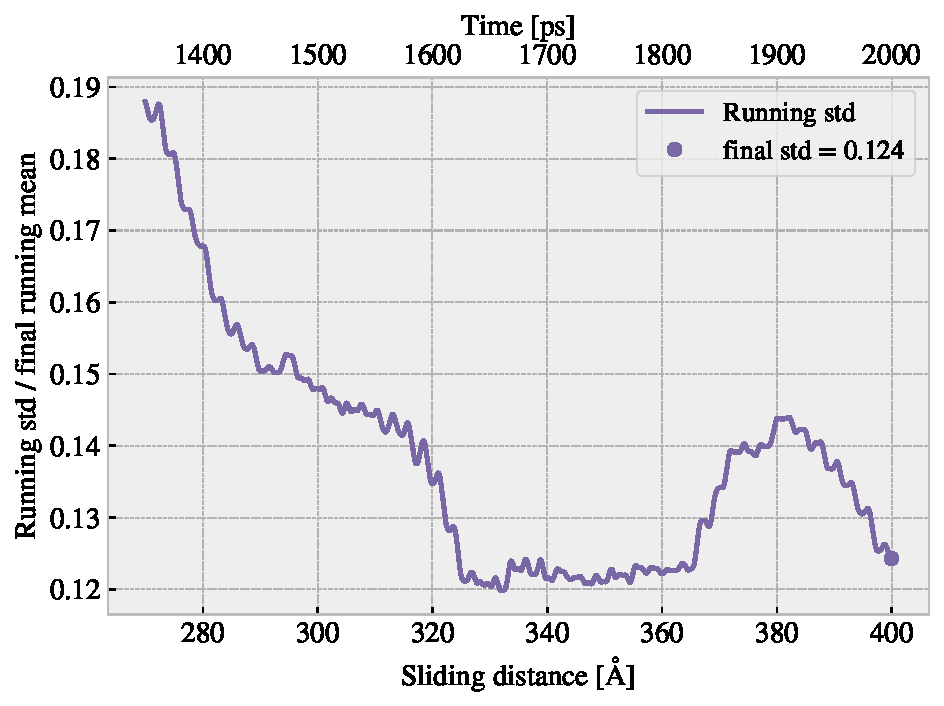
\includegraphics[width=0.6\linewidth]{figures/baseline/Ff_runstd_long.pdf}
  \caption{...}
  \label{fig:runstd_long}
\end{figure}


\paragraph*{Static friction} The max value is the most obvious choice for adressing the static friction, even though that the definition of the static friction is a bit vague. At least when judging from the raw data in figure \ref{fig:drag_Ff} we not see a textbook example of the static friction precourser  (maybe include a classic static friction curve in the theory... I'm not completely sure what to expect here). Additionally the global max value does not always lie in the initial part of the simulation. \\
For a proper static friction evaluation we should increase force slowly and wait for the slip response. Here we drag quite fast making it diffucult to assess the static response. \\
We investigate the placement of the max values, i.e. the drag length for which we measure the max friction force. We show the placement of the top three max values for different simulatiosn with varying normal force in figure \ref{fig:max_dist}. We observe immediately that only a few top three max values is measured within a full slow period of $\sim$ 71 Å. In fact many max values is measured just before the end of the simulation. This indicates that the naive approach of using the overall max value to describe the static friction coefficient might be a to naive approach. Another approach is to use the max value within a single period, but we do not really know if this period will be similar for alle cut patterns and thus this might be limiting. 

\begin{figure}[H]
  \centering
  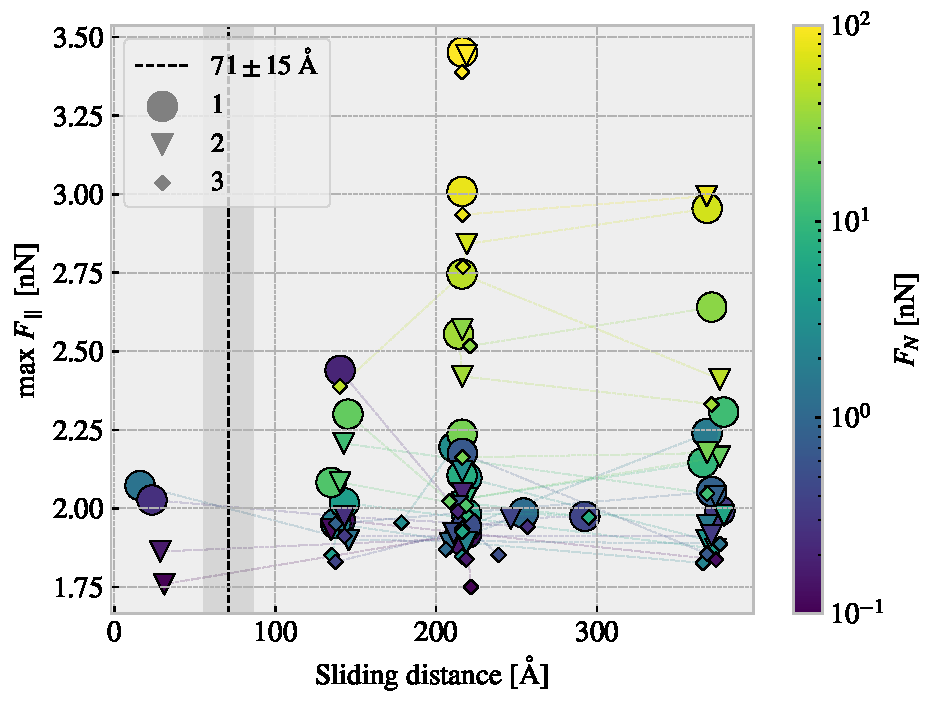
\includegraphics[width=0.6\linewidth]{figures/baseline/max_dist.pdf}
  \caption{Distribution of top 3 max values for different normal force}
  \label{fig:max_dist}
\end{figure}


Look into static friction when having a spring connected to the drag force with
rather low spring constant. Maybe compare to critical sitffness in FK model.
Some rough calculations follow here (make a note about this being a very naive
approach to determine a suitable stiffness for static friction scenarious. In
reality one should increase force slowly to observe this probably). When
dragging the sheet in the y-direction we effectively have a lattice spacing
\begin{align*}
  a_c = a_{2,x} + B_x = a_G\frac{\sqrt{3}}{2} + \frac{a_G}{2\sqrt{3}} = \frac{2a_G}{\sqrt{3}}
\end{align*}
for graphene lattice constant $a_G = 2.46$ Å. For the diamond silicon structure
this is essentially equal to the lattice constant $a_D = 5.4210$ Å. This gives 
\begin{align*}
  \theta = \frac{a_c}{a_b} = \frac{2}{\sqrt{3}}\frac{a_G}{a_D} \approx 0.5230.
\end{align*}
Since we have the factor $2/\sqrt{3}$ it is safe to assume that this is a
irrational number leadning to incommensurability. The worst case scnario of
incommensurability (where $\theta$ equals the golden-mean, Can we get the exact
number?) gives the minimal critical stiffness $K_c \sim 2U_0
(\frac{\pi}{a_b})^2$, where $U_0$ is the substrate potentiual magnitude and
$a_b$ the lattice spacing of the substrate. The potential barrier $U_0$ can be
approximated by the work done when resisting the normal force as $\sim F_N
a_D/2$ such that the critical stiffness can be approximated to 
\begin{align*}
  K_c \sim 2 F_N \frac{a_D}{2} \left(\frac{\pi}{a_D}\right)^2 = \frac{F_N}{a_D}\pi^2
\end{align*}
With a normal force of 1 nN we get $K_c \sim 18$ N/m. Hence, we should try a
spring constant lower than that as qualified way of determining if this is the
reason why we do not really see static friciton in the simulation. 



\newpage
\subsubsection{Varying temperature, drag speed, spring constant and dt}


\begin{figure}[H]
  \centering
  \begin{subfigure}[b]{0.49\textwidth}
      \centering
      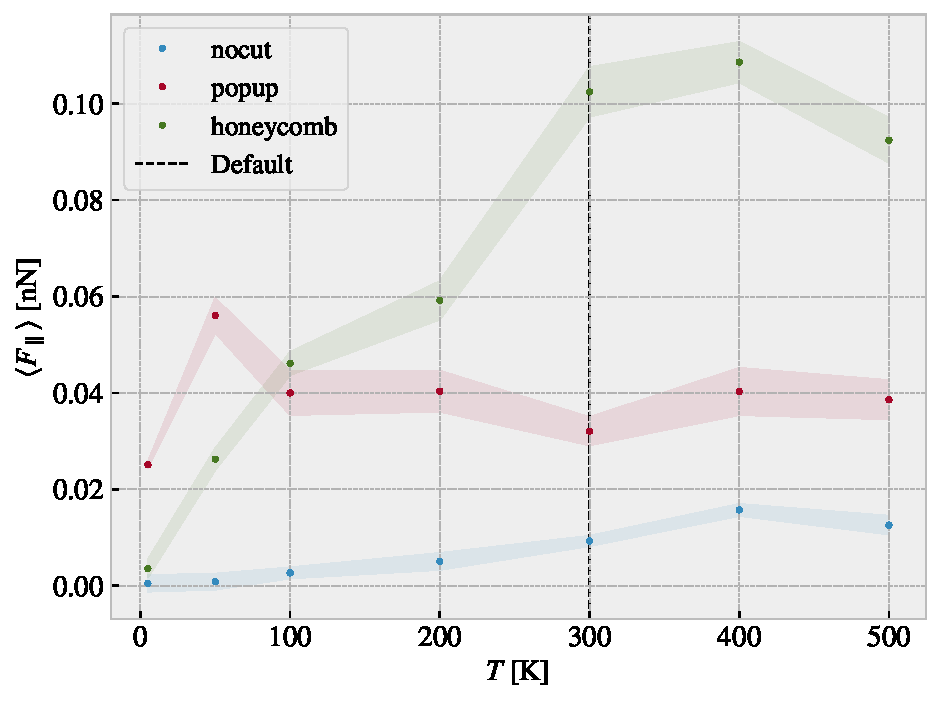
\includegraphics[width=\textwidth]{figures/baseline/variables_temp_mean_fixmove.pdf}
      \caption{mean friction}
      \label{fig:var_temp_mean}
  \end{subfigure}
  \hfill
  \begin{subfigure}[b]{0.49\textwidth}
      \centering
      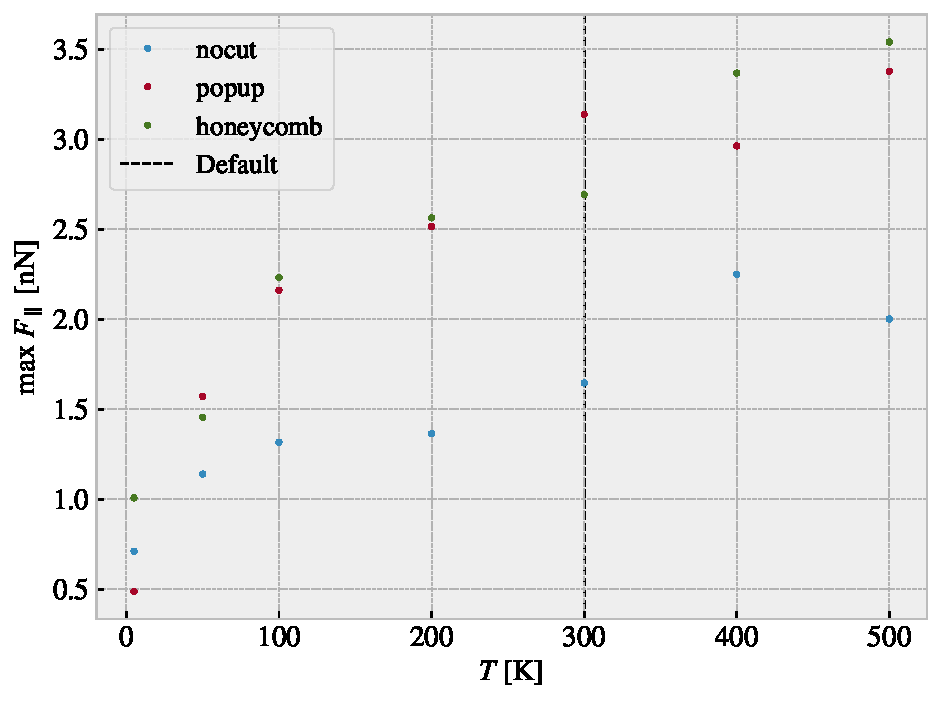
\includegraphics[width=\textwidth]{figures/baseline/variables_temp_max_fixmove.pdf}
      \caption{max friction}
      \label{fig:var_temp_max}
  \end{subfigure}
  \hfill
     \caption{Temperature}
     \label{fig:var_temp}
\end{figure}

\begin{figure}[H]
  \centering
  \begin{subfigure}[b]{0.49\textwidth}
      \centering
      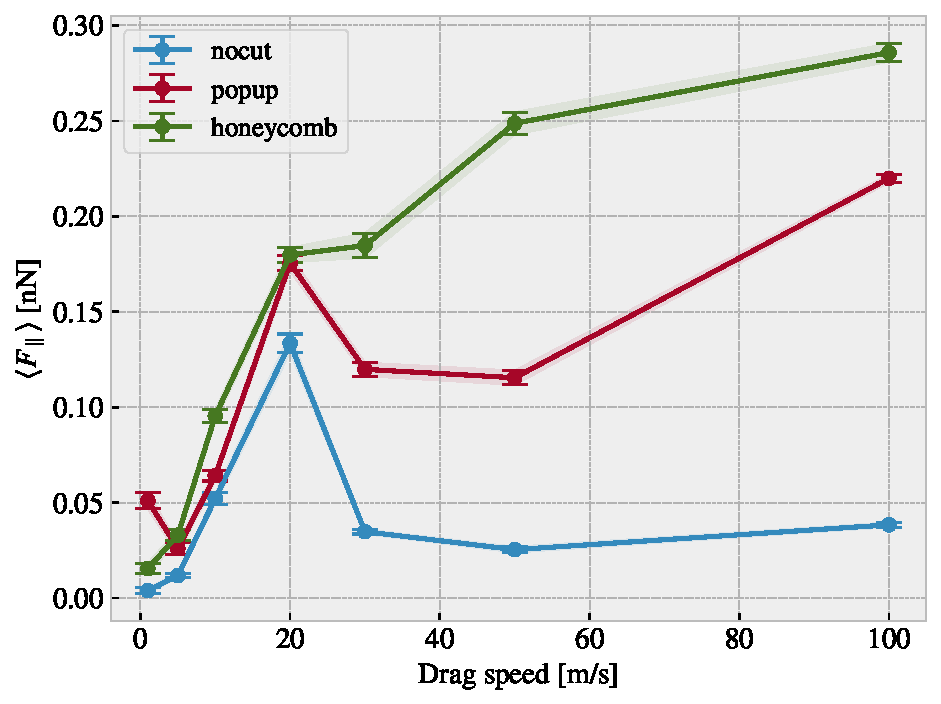
\includegraphics[width=\textwidth]{figures/baseline/variables_vel_mean_K30.pdf}
      \caption{mean friction}
      \label{fig:var_vel_mean}
  \end{subfigure}
  \hfill
  \begin{subfigure}[b]{0.49\textwidth}
      \centering
      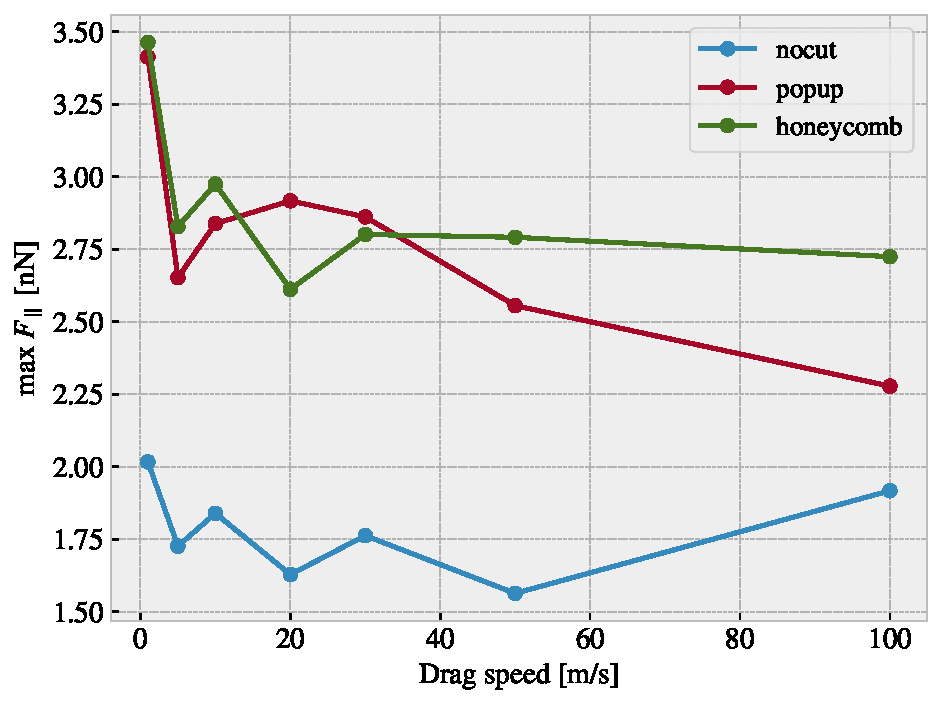
\includegraphics[width=\textwidth]{figures/baseline/variables_vel_max_K30.pdf}
      \caption{max friction}
      \label{fig:var_vel_max}
  \end{subfigure}
  \hfill
     \caption{Drag speed}
     \label{fig:var_vel}
\end{figure}


Simulations of concentric nanotubes in relative motion (telescopic sliding), have revealed the occurrence of well-defined velocities at which friction is enhanced, corresponding to a washboard frequency resonating with longitudinal [172] or circular [173] phonon modes, leading to enhanced energy dissipation. The frictional response becomes highly non-linear while approaching the critical velocity and, contrary to macroscopic systems, washboard resonances can arise at multiple velocities, especially for incommensurate interfaces where more than one length scale may be in common to the contacting surfaces [172] \cite{Manini_2016}.


\begin{figure}[H]
  \centering
  \begin{subfigure}[b]{0.49\textwidth}
      \centering
      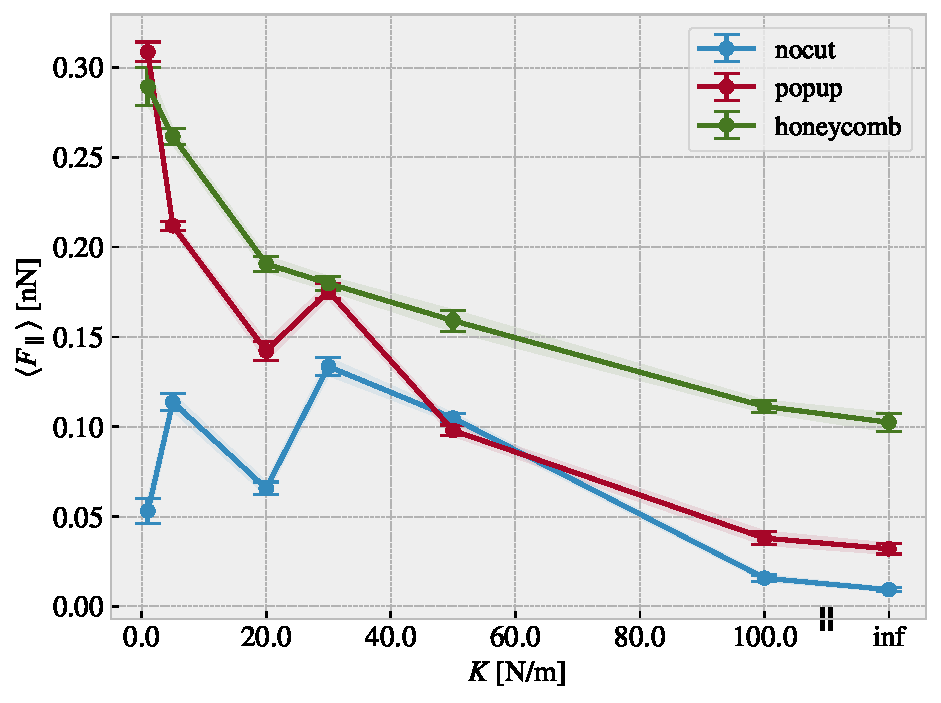
\includegraphics[width=\textwidth]{figures/baseline/variables_spring_mean_K30.pdf}
      \caption{mean friction}
      \label{fig:var_K_mean}
  \end{subfigure}
  \hfill
  \begin{subfigure}[b]{0.49\textwidth}
      \centering
      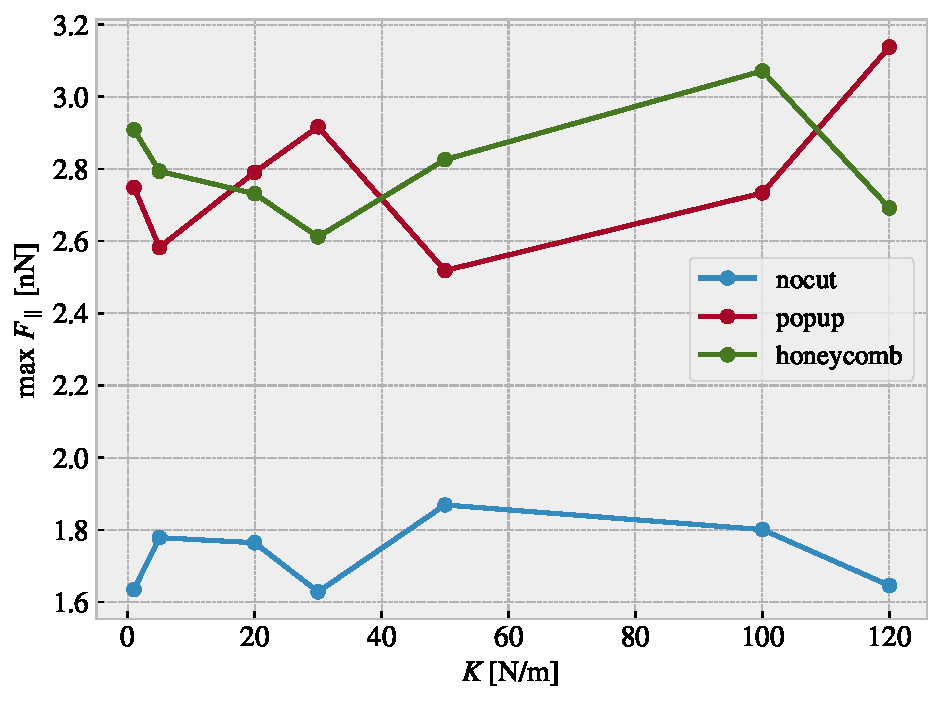
\includegraphics[width=\textwidth]{figures/baseline/variables_spring_max_K30.pdf}
      \caption{max friction}
      \label{fig:var_K_max}
  \end{subfigure}
  \hfill
     \caption{Spring constant}
     \label{fig:var_K}
\end{figure}

\begin{figure}[H]
  \centering
  \begin{subfigure}[b]{0.49\textwidth}
      \centering
      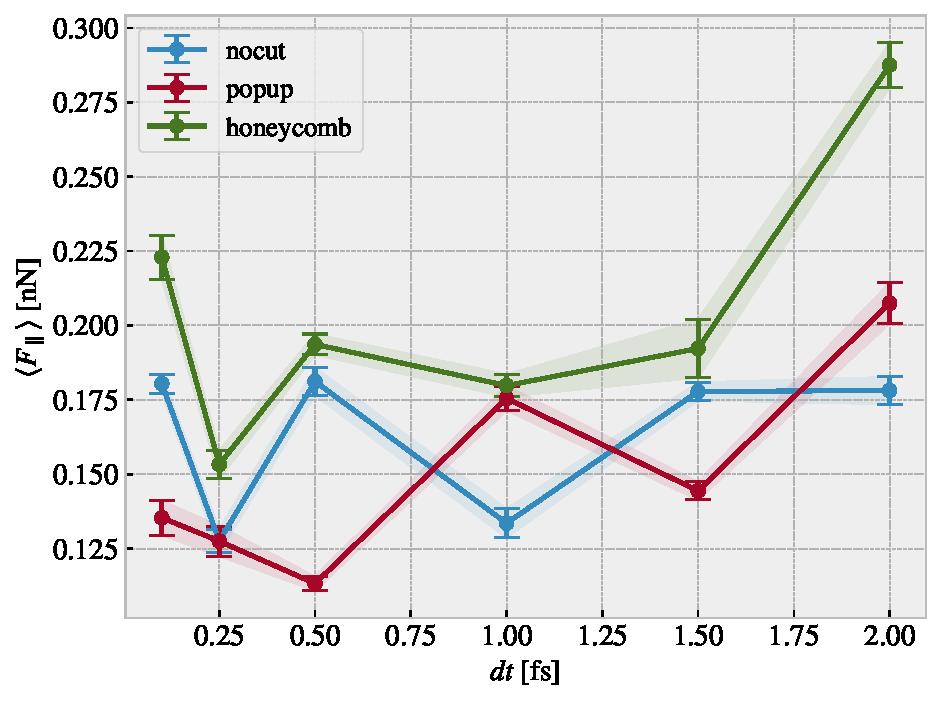
\includegraphics[width=\textwidth]{figures/baseline/variables_dt_mean_K30.pdf}
      \caption{mean friction}
      \label{fig:var_dt_mean}
  \end{subfigure}
  \hfill
  \begin{subfigure}[b]{0.49\textwidth}
      \centering
      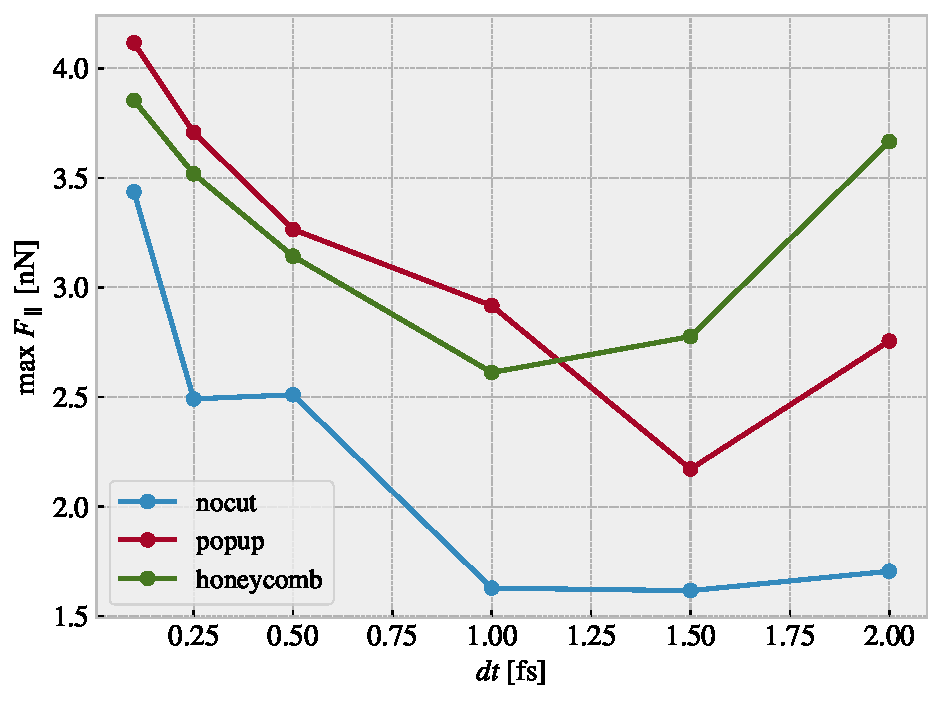
\includegraphics[width=\textwidth]{figures/baseline/variables_dt_max_K30.pdf}
      \caption{max friction}
      \label{fig:var_dt_max}
  \end{subfigure}
  \hfill
     \caption{Timestep}
     \label{fig:var_dt}
\end{figure}




\newpage
\subsubsection{Varying normal force and stretch}
\paragraph*{Multi stretch} 
text

\begin{figure}[H]
  \centering
  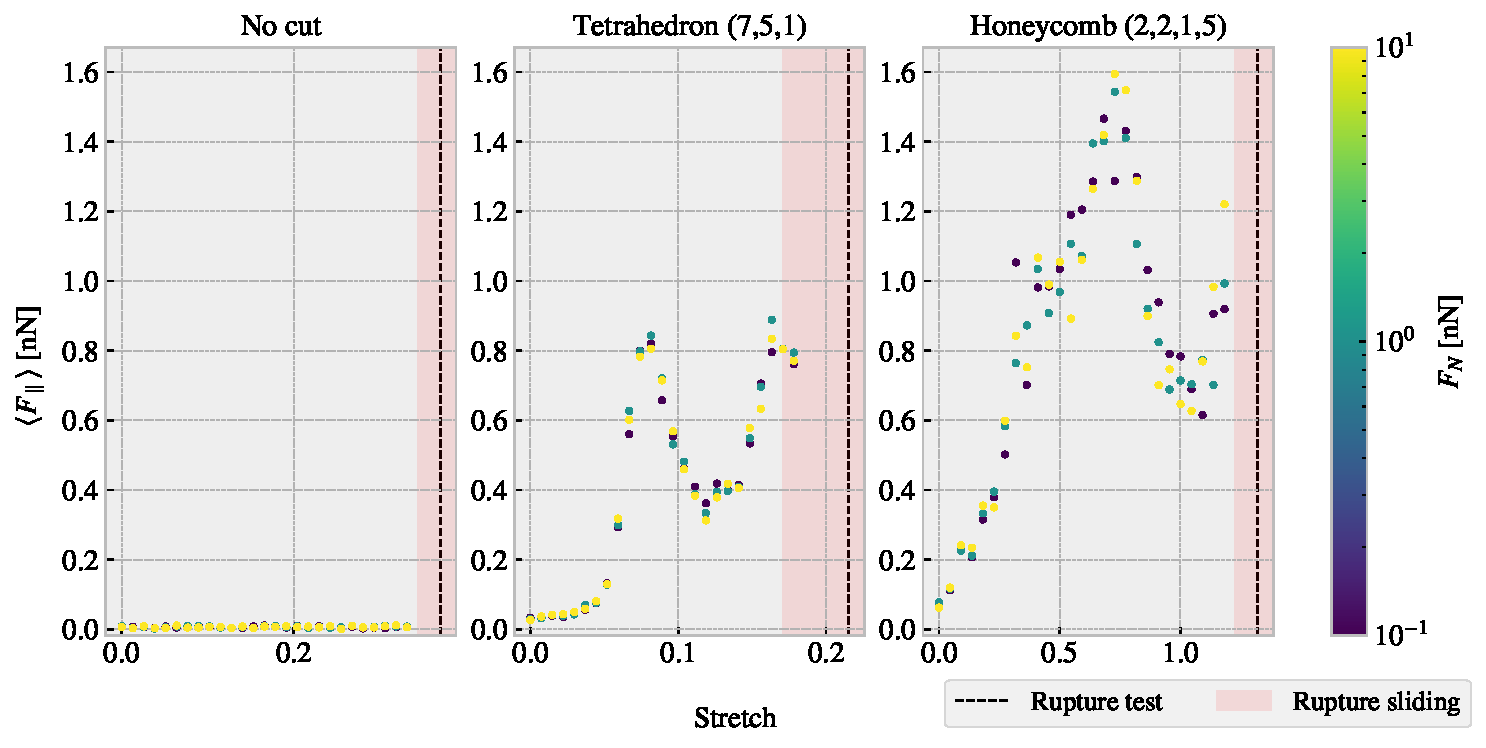
\includegraphics[width=\linewidth]{figures/baseline/multi_stretch_mean_compare.pdf}
  \caption{...}
  \label{fig:}
\end{figure}


\begin{figure}[H]
  \centering
  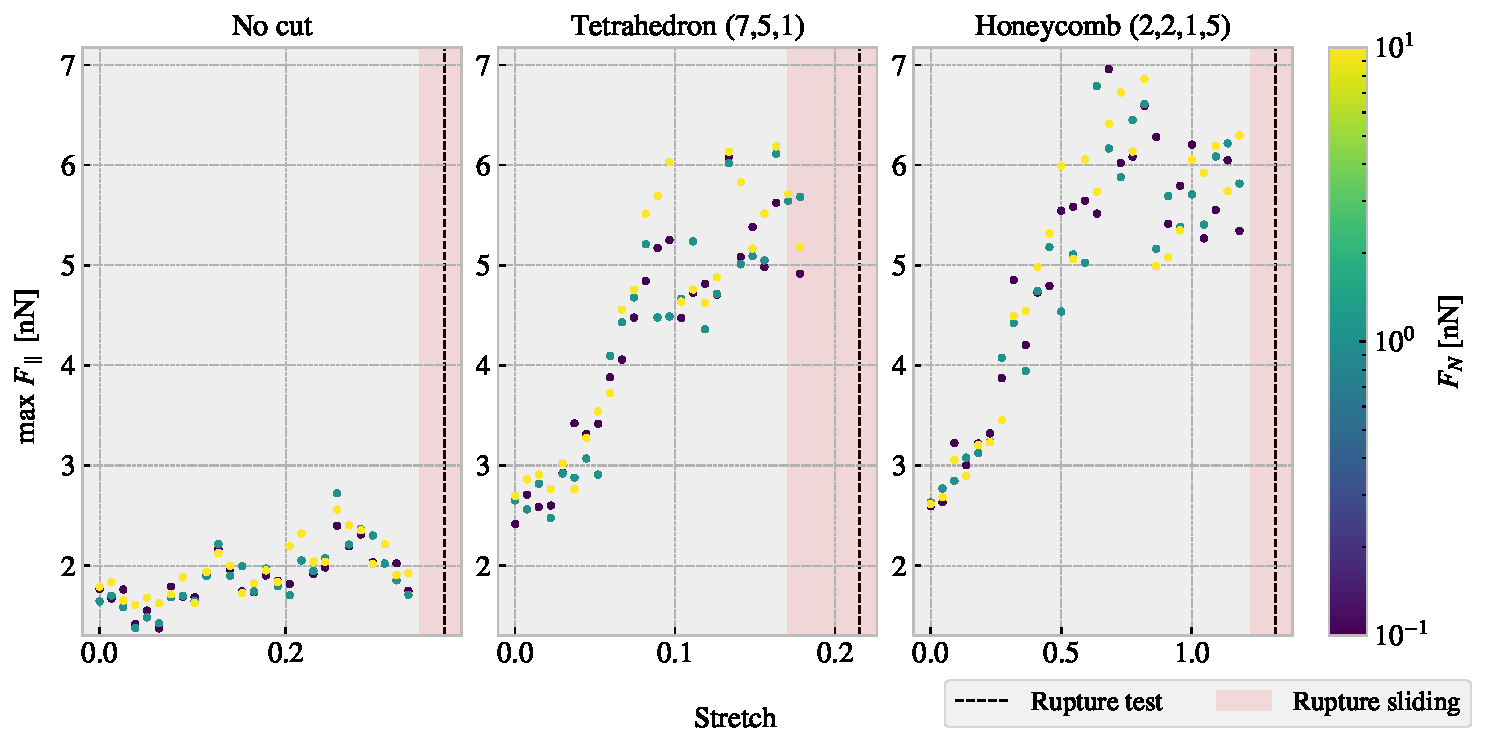
\includegraphics[width=\linewidth]{figures/baseline/multi_stretch_max_compare.pdf}
  \caption{...}
  \label{fig:}
\end{figure}

\paragraph*{Multi normal force}



\begin{figure}[H]
  \centering
  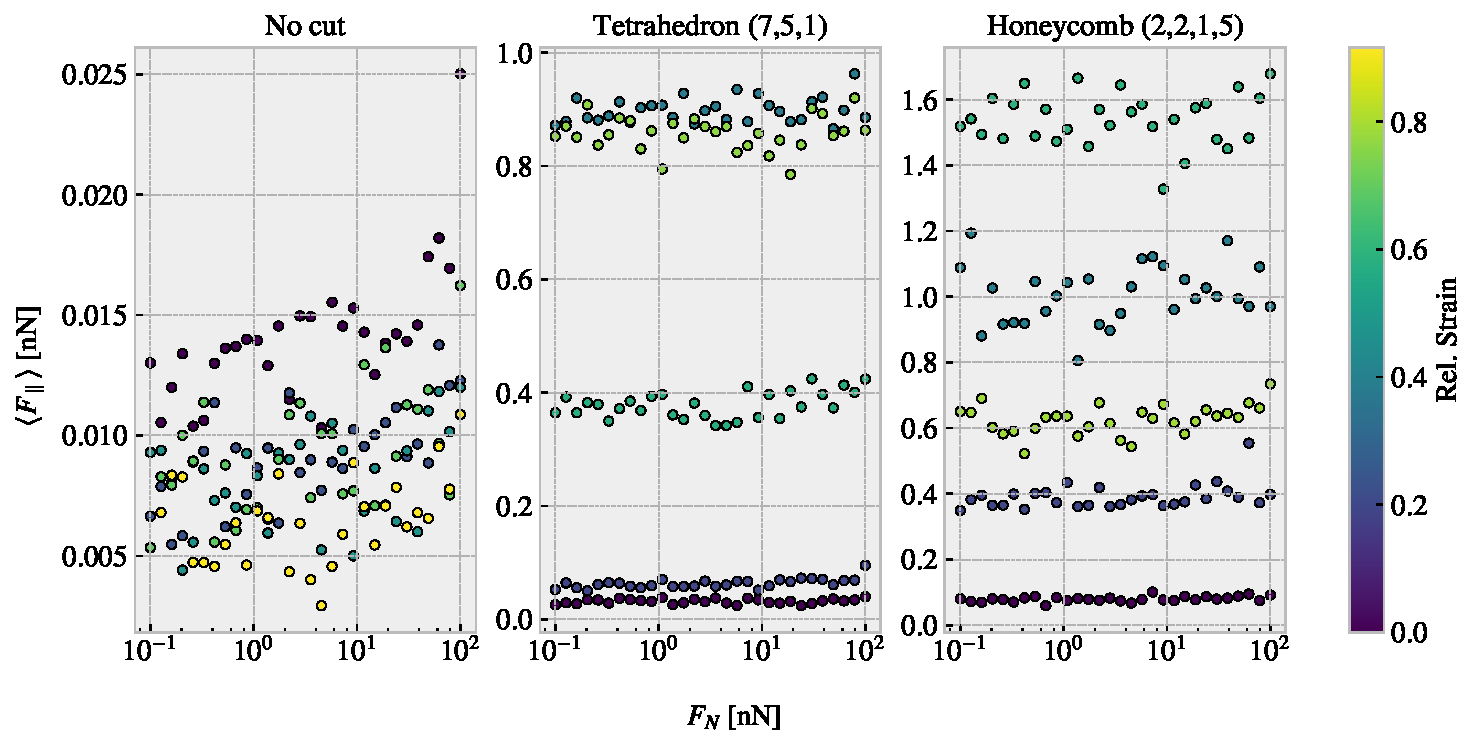
\includegraphics[width=\linewidth]{figures/baseline/multi_FN_mean_compare.pdf}
  \caption{...}
  \label{fig:}
\end{figure}


\begin{figure}[H]
  \centering
  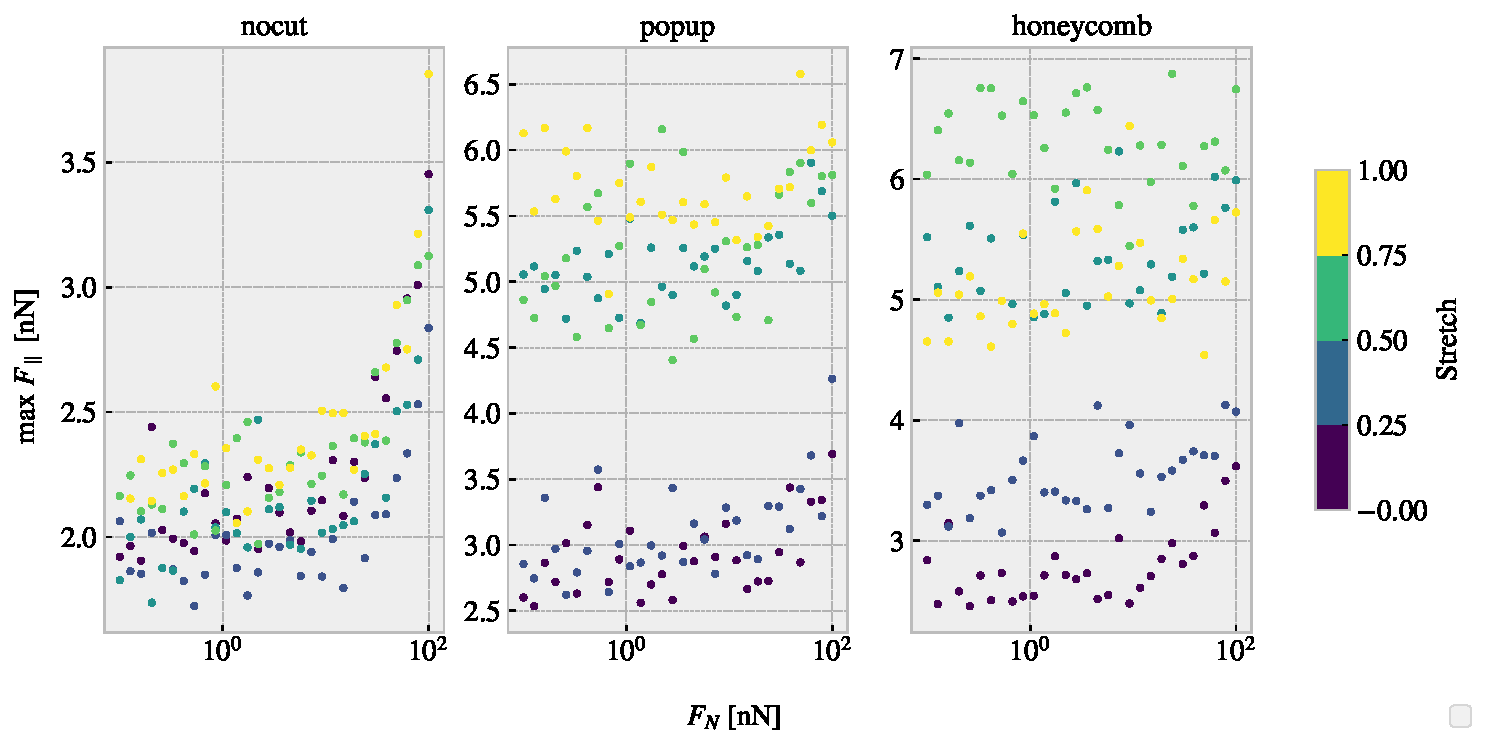
\includegraphics[width=\linewidth]{figures/baseline/multi_FN_max_compare.pdf}
  \caption{Colorbar is only fitted for the right plot (honeycomb)... this should be fixed. Should I have run a linear distribtion of FN so I could plot it linear here also...?}
  \label{fig:}
\end{figure}



\begin{table}[H]
  \begin{center}
  \caption{Mean friction coeff}
  \label{tab:fric_coeff}
  \begin{tabular}{| c | c | c | c | c | c |} \hline
    nocut & 0.00009 $\pm\num{1e-05}$ & 0.00005 $\pm\num{1e-05}$ & 0.00004 $\pm\num{1e-05}$ & 0.00005 $\pm\num{2e-05}$ & \\ \hline
    popup & 0.00005 $\pm\num{3e-05}$ & 0.00024 $\pm\num{5e-05}$ & 0.0002 $\pm\num{2e-04}$ & 0.0005 $\pm\num{1e-04}$ & 0.0003 $\pm\num{2e-04}$ \\ \hline
    honeycomb & 0.00013 $\pm\num{6e-05}$ & 0.0006 $\pm\num{3e-04}$ & 0.0004 $\pm\num{6e-04}$ & 0.0007 $\pm\num{6e-04}$ & 0.0009 $\pm\num{3e-04}$ \\ \hline
  \end{tabular}
  \end{center}
\end{table}

\begin{table}[H]
  \begin{center}
  \caption{Max friciton coeff}
  \label{tab:fric_coeff}
  \begin{tabular}{| c | c | c | c | c | c |} \hline
    nocut & $0.0139 \pm \num{9e-04}$& $0.0083 \pm \num{7e-04}$& $0.010 \pm \num{1e-03}$& $0.0105 \pm \num{9e-04}$ &  \\ \hline
    popup & $0.007 \pm \num{2e-03}$& $0.010 \pm \num{2e-03}$& $0.007 \pm \num{2e-03}$& $0.009 \pm \num{3e-03}$& $0.006 \pm \num{2e-03}$ \\ \hline
    honeycomb & $0.010 \pm \num{1e-03}$& $0.007 \pm \num{2e-03}$& $0.007 \pm \num{3e-03}$& $0.000 \pm \num{3e-03}$& $0.004 \pm \num{3e-03}$ \\ \hline
  \end{tabular}
  \end{center}
\end{table}


The friction probably does not increase with normal force at an expected rate due to the fact the normal force is only applied on the pull blocks. Especially with the cutted sheet the tension drops such that the effecive normal force on the inner sheet is not changing so much. By this theory the friction force vs. normal force on the pull graph look a bit more like expected.

When looking at the graphs for the PB the max friction is visually textbook linear, while the mean friction is a bit more linear but also with negativ coefficients.

\subsubsection{Contact area}

Show plots of contact area vs stretch and discuss the fact that friction actually increases while contact area drops. Is the conclusion that there might be another more dominant cause of the increasing friction. 

\begin{figure}[H]
  \centering
  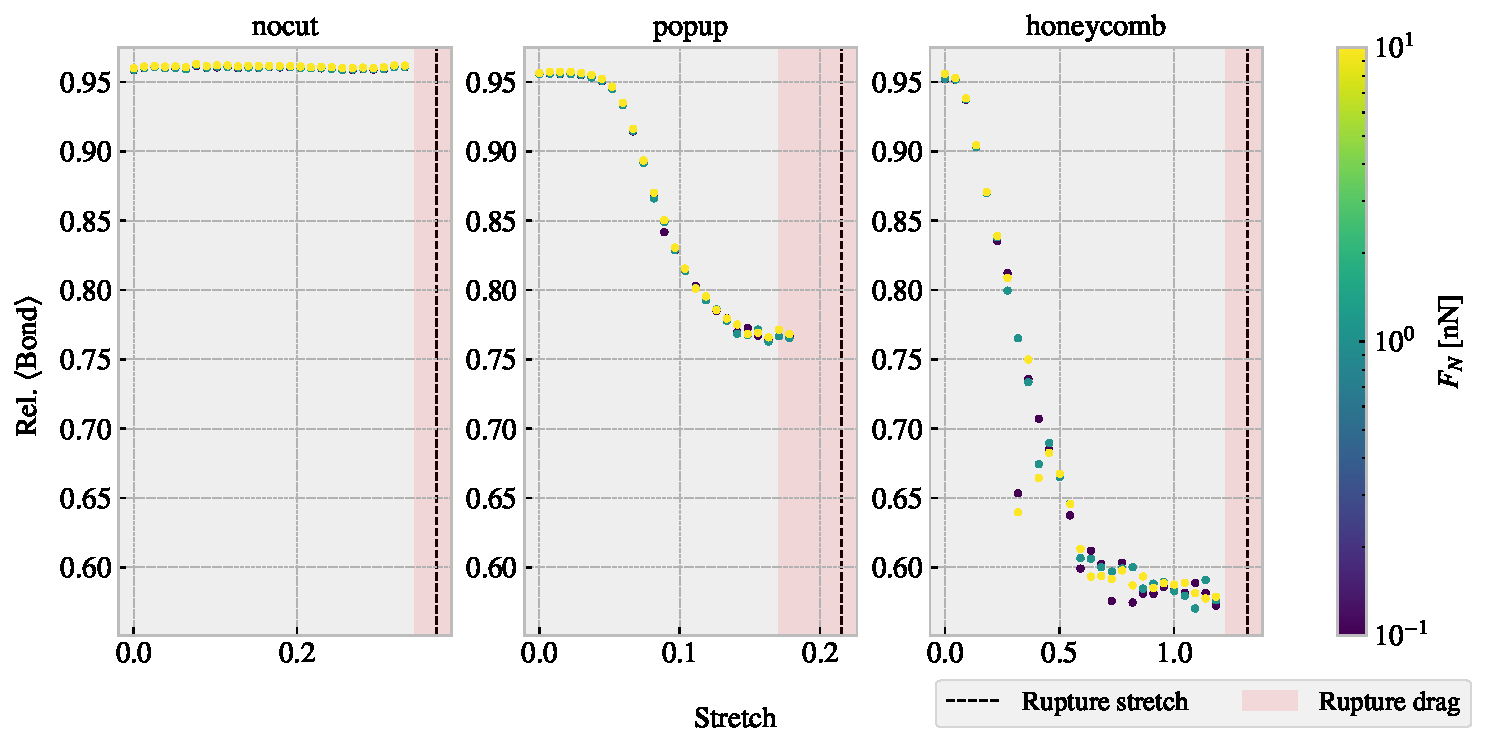
\includegraphics[width=\linewidth]{figures/baseline/multi_stretch_area_compare.pdf}
  \caption{}
  \label{fig:}
\end{figure}
